System virtualization is a way for a data center to reduce cost and power by overcommitting and sharing system resources across disparate operating systems with common hardware.  Since each guest machine only uses a portion of the available resources at any given time, the total resources allocated to all guest VMs can exceed the total physical resources \cite{huber2, amit, buell1}.   This idea of overcommitting resources is the same as preemptive multitasking, where multiple processes share a single CPU; and OS virtual memory, where the total memory available to applications exceeds the physical memory capacity.   

\indent Due to these cost savings and decreased physical administration overhead, IT Data Centers and Businesses are moving toward virtualized environments.  In 2008 Gartner’s showed that 12\% of hardware at data centers were virtualized, and then predicted that by 2013 61\% would be virtualized \cite{gartners}.   Additionally, research from Ramya and Edwin show tremendous growth in Platform As A Service (PAAS) where an entire system platform is dynamically provisioned in a cloud computing service \cite{ramya}.   Massive data centers are able to provide virtual systems, and manage large clusters of shared resources, for a fraction of the price of building a physical server for each customer.

\begin{figure}[!b]
  \begin{center}
    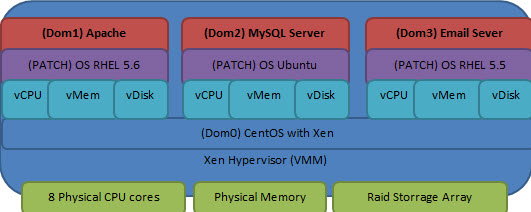
\includegraphics[width=3.5in]{images/VirtualizationExample.jpg}
  \end{center}

  \caption{\small In this example there are 3 paravirtualized guests (DomU) running on a Xen Server.  The Xen hypervisor and Dom0 divide, share, and overcommit the physical resources between the 3 guest domains.  Each guest has access to virtual resources and not physical hardware.}
  \label{virtStack}
\end{figure}

\indent The problem virtualization introduces is profiling and analysis of this additional layer of abstraction for the guest systems.  The hypervisor, or Virtual Machine Manager, adds to the already complex existing layers (Application, OS, and Hardware) one must analyze when an application performs sub-optimally.  How can a system administrator determine if the problem is in the application, OS, hypervisor, hardware, or an unrelated guest virtual machine on the same physical host system?  In a single server environment or HPC cluster there can be 'interference' \cite{paul} or ‘system noise' caused by these layers, which contributes to poor application performance.  The hypervisor as well as multiple other guest virtual machines (See: figure \ref{virtStack}) compete for system resources and add to this interference.  Addtional information is needed, in order for a running guest application to accurately analyze this interference.

\indent This research shows a method for analyzing performance data at runtime in the guests and Virtual Machine Monitor (VMM).   With this framework we are now able to determine the layer of the complex software stack and the detect the interference and overhead from virtualization.  Additionally, we can determine which system resource (memory, CPU, or IO) needs to be modified or is used inefficiently.  This could significantly reduce time spent troubleshooting and analyzing performance problems in virtualized environments.

\indent This project will add the following contributions for virtualization:
\begin{enumerate}
\item Define the layers of abstraction in virtual environments.
\item Define the system resources which attributes to application problem from I/O, memory, or CPU problems.
\item Framework to identify the counters, metrics, and environment at each layer.
\item Virtualization test suite that causes I/O interference in several different areas.
\item Example tool which dynamically analyzes runtime interference and identifies the layer which experiences I/O contention.
\item Introduce \emph{disk pinning} for virtualization where separate physical disks are assigned to individual virtual servers.
\end{enumerate}

\indent The rest of this document is organized as follows:  In section 2, we look at a real problem example in a large data center, and the challenges faced with existing tools.  In section 3, we examine the current state of tools and techniques used to profile and analyze performance issues with virtualization.  Section 4 looks at related works that have identified interference and methods of root cause analysis.  In section 5 we define the needed data and an example tool that can collect and analyze this data.  The last sections are dedicated to the test suite infrastructure to both create the interference and show the accuracey of the analysis.  We also look at possible other uses and what needs further investigation.
